%!TEX root=./LIVRO.tex
\captionsetup{font={small, it}}
\captionsetup{justification=raggedright, singlelinecheck=false}

\chapter{Apresentação da plataforma}

% Odoo em Portugal, características técnicas (eLeading, Survey)

A plataforma foi desenvolvida com base em um sistema integrado de gestão 
de código aberto e abrangente\footnote{O nome do sistema é Odoo, um conjunto belga de ferramentas 
de \textit{software} de gestão que inclui, por exemplo, CRM, \textit{e-commerce}, faturamento, 
contabilidade, manufatura, armazém, gerenciamento de projetos e gerenciamento 
de estoque, além de ferramentas de ensino e pesquisa.}.

Desenvolvido inicialmente em 2005, o sistema oferece uma ampla gama de módulos e 
recursos que podem ser personalizados e adaptados às necessidades específicas de 
diferentes tipos de empresas e setores. Ele é construído sobre uma arquitetura 
modular, o que significa que os usuários podem selecionar e implementar apenas 
os módulos relevantes para suas operações.

Possui uma interface amigável e intuitiva, facilitando a navegação e a 
utilização do sistema. Além disso, sua natureza de código aberto permite que 
desenvolvedores personalizem e estendam o \textit{software} para atender às demandas 
específicas de cada negócio.

O mesmo sistema é usado em escolas de Portugal, o que representa a maior implementação 
desse sistema no mundo. Serviços como gestão de recursos humanos, recrutamento e avaliação 
anual de professores foram adaptados para o uso do sistema.

\subsection{eLearning e Survey}

O sistema oferece recursos relacionados ao \textbf{eLearning} e à aplicação de questionários. 
Esses recursos podem ser úteis para instituições educacionais, empresas que oferecem treinamentos 
\textit{on-line} ou qualquer organização que deseje criar cursos e compartilhar conhecimento

\begin{enumerate}
\item O módulo chamado eLearning permite a criação e o gerenciamento de cursos \textit{on-line}. Com ele, 
é possível criar conteúdo educacional, como vídeos, documentos, questionários, e disponibilizá-lo 
aos alunos para que possam acessar e aprender no próprio ambiente. O módulo também permite o 
acompanhamento do progresso dos alunos, a atribuição de certificados, fóruns de discussão e outras 
interações relacionadas ao aprendizado.

\item O módulo Survey permite a criação e a condução de pesquisas. Com essa funcionalidade, podem-se criar 
questionários personalizados com diferentes tipos de pergunta (múltipla escolha, texto aberto, escalas etc.), 
compartilhá-los com os participantes e coletar as respostas. Além disso, os resultados podem ser analisados 
por meio de gráficos e relatórios integrados.
\end{enumerate}

\begin{figure}[t]
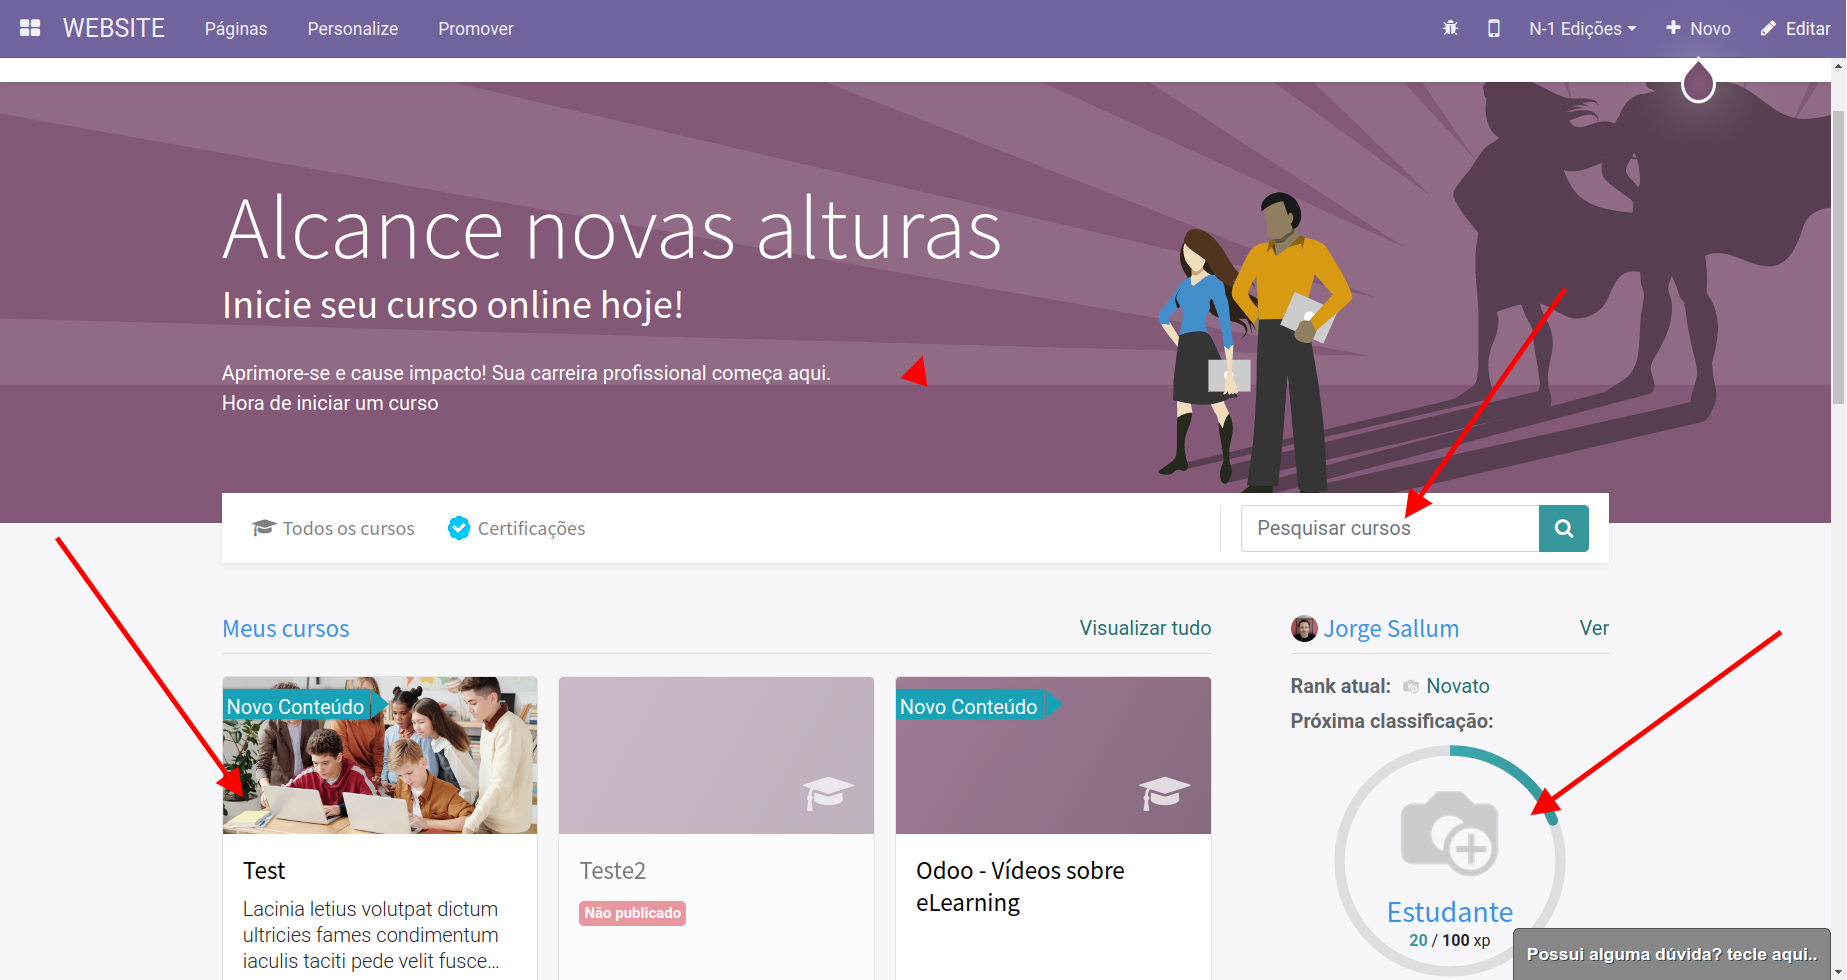
\includegraphics[width=\textwidth]{imgs/screenshot1}
\end{figure}


\section{A quem se destina}
% Felipe

A plataforma da coleção Revisa SAEB destina-se a alunos e professores do 1º ao 9º ano 
do Ensino Fundamental.

Por meio dela, os alunos têm acesso às versões digitais do material impresso, dos testes da seção 
chamada Treino e dos simulados, além de vídeos e jogos. Já os professores, além de terem acesso ao 
mesmo conteúdo que os alunos, acessam uma série de vídeos de capacitação e podem acompanhar o 
desempenho dos estudantes.

% Quantos cursos, como estão dividas as seções, natureza dos conteúdo

\section{Como acessar?}

% Jorge

\lipsum[1-3]
\begin{figure}[t]
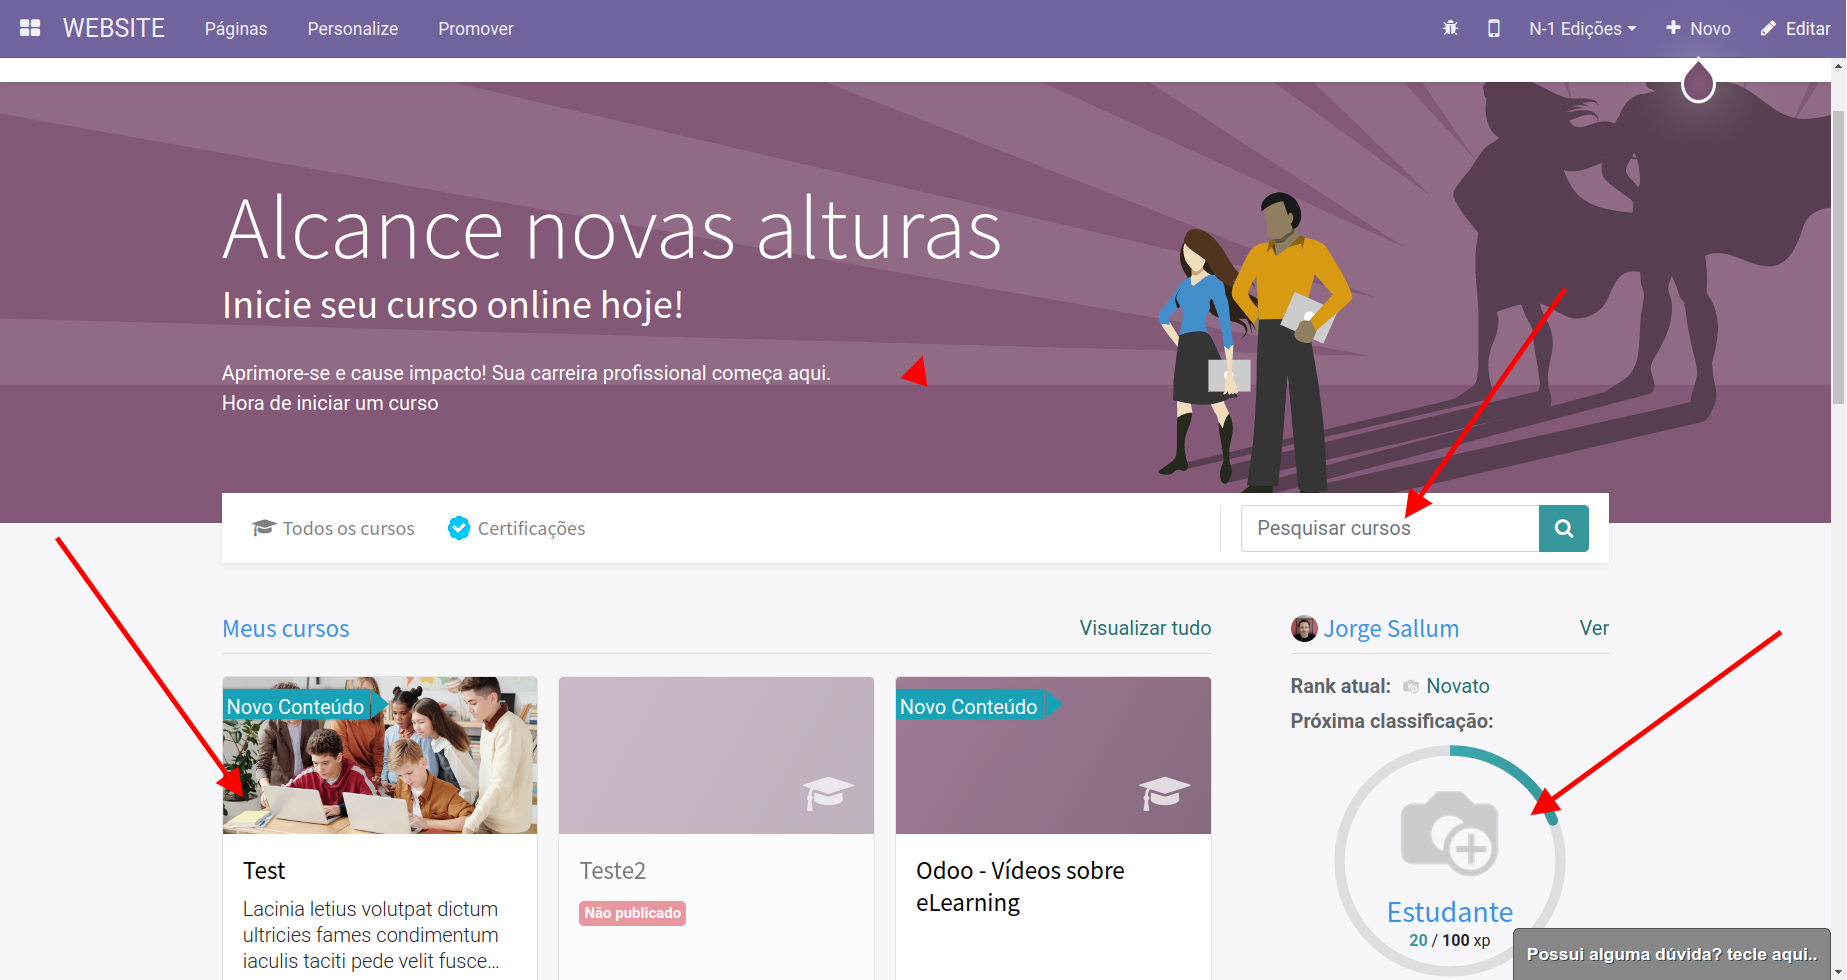
\includegraphics[width=\textwidth]{imgs/screenshot2}
\end{figure}

\section{Apresentação do conteúdo digital}

% André
% Explicar as seções, a relação com o material impresso, os quiz

\lipsum[1-3]

\section{Estrutura do site} % Jorge




